\documentclass{article}
\usepackage{amsmath}
\usepackage[a4paper, top=1in, bottom=1in, left=0.75in, right=0.75in]{geometry}
\usepackage{graphicx}
\usepackage[hidelinks]{hyperref}
\usepackage[style=ieee, giveninits=false]{biblatex}

\addbibresource{references.bib}

\graphicspath{{./images/}}

\title{Addressing Limitations in 3D Hand-Object Interaction with HOISDF}
\author{David Robinson}
\date{}
\setlength{\parskip}{1em}

\pagenumbering{gobble}

\begin{document}

\maketitle

\section*{Introduction}

The HOISDF model~\cite{qi2024hoisdf} predicts the 3D hand and object keypoints from a single RGB image for hand-object interactions and was accepted by CVPR 2024. It first estimates signed distance fields~\cite{ma2021neuralpull} for both the hand and object to build the shape of each with sampled points. A signed distance field is a scalar field that represents the shortest difference from any point in a 3D space to the surface, where the sign indicates whether the point is inside (negative) or outside (positive) the object. The sampled points on the surface are then used to predict the hand joints and shape, as well as the object's position and orientation in the image.

\begin{center}
    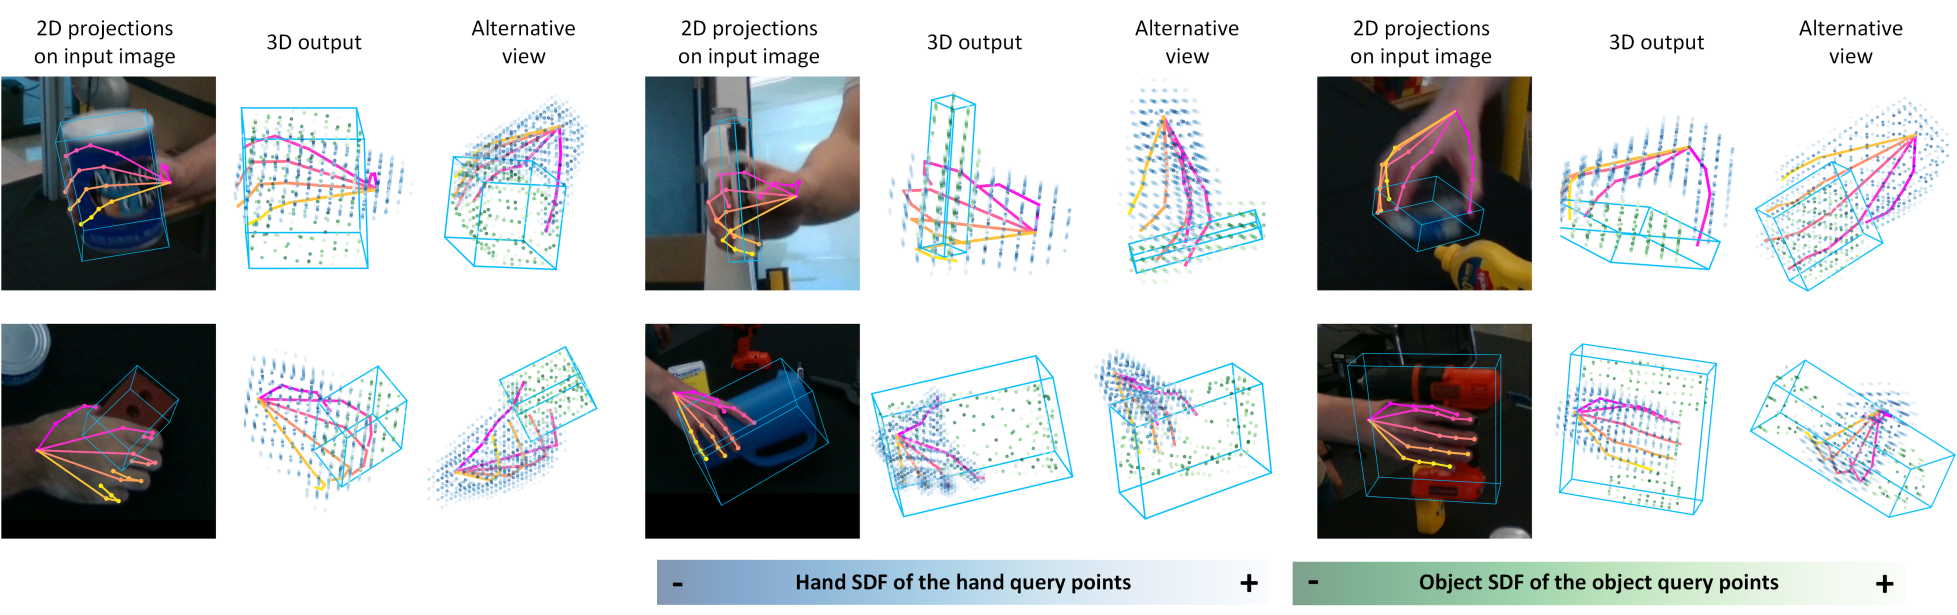
\includegraphics[scale=0.25]{hoisdf-1.png}
\end{center}

\section*{Background}

3D pose estimation is the field of estimating 3D coordinates of keypoints or joints from various input data, such as 2D images, depth maps, or WiFi signals. This technology plays a critical role in fields like robotics~\cite{billard2019robotics}, augmented reality~\cite{chen2019augmentedreality}, and healthcare~\cite{stenum2021health}, where precise tracking and analysis of movement are essential.

One category of pose estimation with an RGB image is regression-based methods, where the 3D coordinates are regressed from the input image. For example, the ResNet~\cite{he2016resnet} model passes the input image through convolution layers to generate features and then those features are regressed to the 3D coordinates using a fully connected layer. Heatmap-based methods, such as EgoTAP~\cite{kang2024egotap}, are also very common where a heatmap of the 2D coordinates is predicted first and then a separate network directly lifts them to 3D. This method does not perform as well in occluded scenarios because it depends on the accuracy of the 2D coordinates and does not use context from the original image. Also, there is ambiguity in the projection as there are multiple possible ways to lift a set of 2D coordinates to 3D~\cite{zhou2024lifting}.

\section*{Motivation}

Estimating the 3D poses of a hand and an object from a single camera is challenging due to the frequent occlusions during interaction. Most existing methods struggle in these scenarios because they rely on limited shape information or explicit representations like meshes, which only provide local context. Direct lifting methods predict 3D poses directly from 2D image features, without intermediate 3D representations, depending entirely on the network's ability to learn the 2D-to-3D mapping, making them less robust to occlusions~\cite{kang2024egotap}. Coarse-to-fine methods refine an initial prediction of the 3D joints or shape, but the reliance on explicit 3D representations often fails to capture global context~\cite{cheng2024handdiff}. Unlike explicit representations, signed distance fields provide a global, continuous, and implicit representation of the 3D shapes across the entire 3D volume. Signed distance fields not only encode the shape of the hand and object, but also their interactions and collision points, providing a way to address occlusions and provide global constraints for the 3D pose.

\begin{center}
    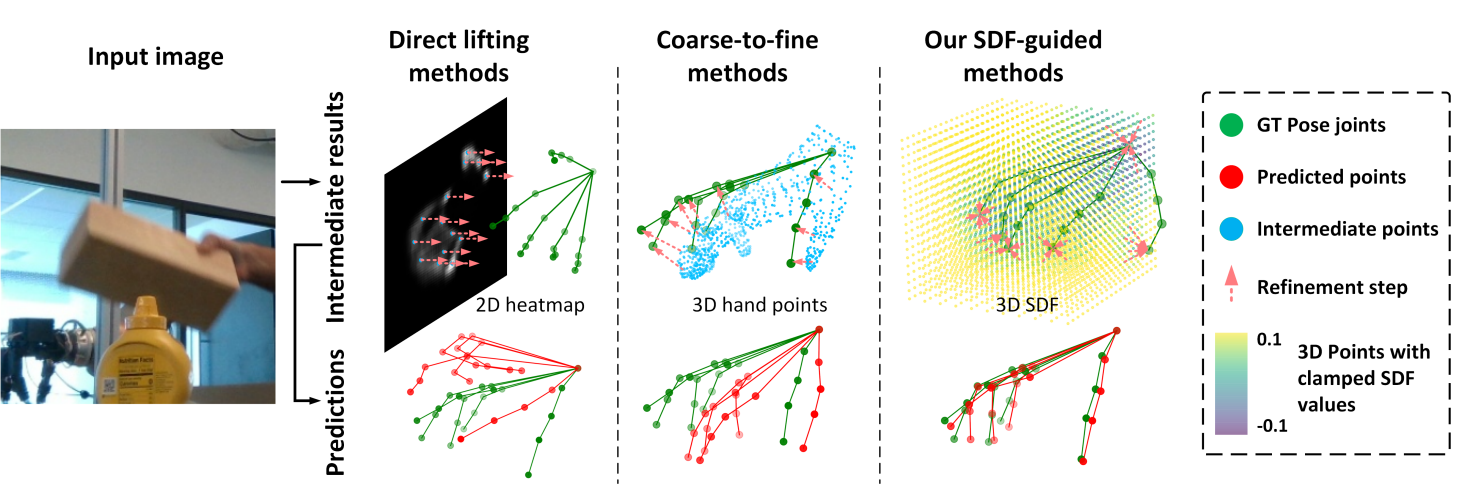
\includegraphics[scale=0.4]{hoisdf-2.png}
\end{center}

\begin{center}
    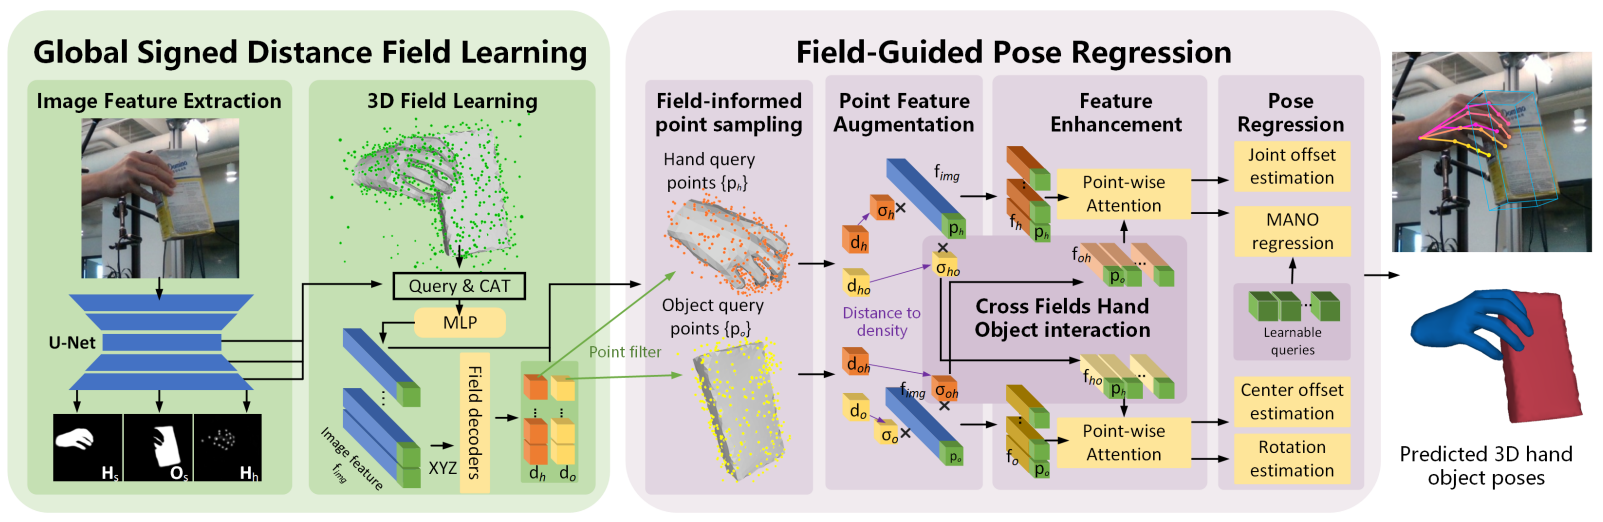
\includegraphics[scale=0.4]{hoisdf-3.png}
\end{center}

\section*{Method}

\subsubsection*{Signed Distance Field}

A U-Net~\cite{ronneberger2015unet} model extracts the hand and object segmentation masks and 2D keypoint predictions from the image. The decoder part of the U-Net and a multi-layer perceptron (MLP) is used to convert a 3D point into an image feature vector. Fourier positional encoding~\cite{tancik2020fourier} is also incorporated to expand the 3D point to a larger space. The signed distance decoder is a fully connected neural network that predicts the signed distance to the hand or object surface from the 3D point, image features, and positional encodings.

\subsubsection*{Feature Extraction}

The 3D space is divided into a set of 3D bins, each containing a query point. These points are filtered in the 2D space using the hand and object bounding boxes. The filtered set of points are sorted based on their distances to the surface and only the closest points are kept. For each query point, its volume density $\sigma = \alpha^{-1}\text{sigmoid}(-d/\alpha)$, where $\alpha$ is a learned parameter, is calculated where a higher density is closer to the surface, giving more importance to those points. These densities are combined with the query point, positional encodings, and image features, to form the final hand feature vector.

To incorporate hand-object interactions, the object query points are passed through the hand signed distance field to calculate the hand-object distances. These distances, along with the object query points, positional encodings, and image features, are used to form the cross-field hand feature vector.

Since both the final and cross-field feature vectors mainly contain local information, they are passed through six Multi-Head Self-Attention (MHSA)~\cite{vaswani2017attention} layers to incorporate global shape information and form the enhanced hand features. The same process is repeated with the object query points to generate enhanced object features.

\subsubsection*{Pose Regression}

The enhanced hand features are passed through Cross-Attention layers with 17 learned hand pose queries to regress the 3D hand joints and shape~\cite{hampali2022keypointtransformer}. Since the object is more rigid, the rotation and translation vectors, that define the orientation and position of the object, are directly regressed from the enhanced object features.

\begin{center}
    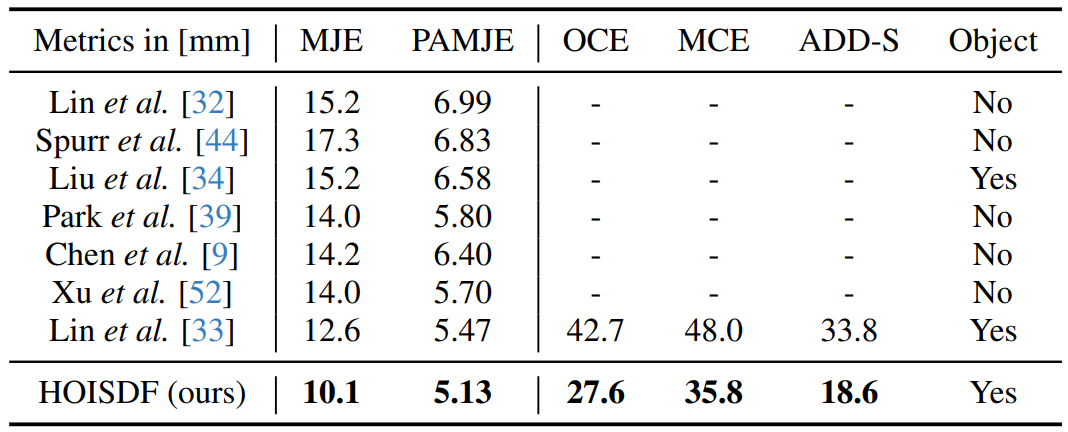
\includegraphics[scale=0.3]{hoisdf-4.png}
\end{center}

This table compares HOISDF~\cite{qi2024hoisdf} against previous state-of-the-art (SOTA) models on the DexYCB~\cite{chao2021dexycb} dataset. The two major metrics are Mean Joint Error (MJE) and Poscrustes-Alignment Mean Joint Error (PAMJE)~\cite{zimmermann2017handpose}, where HOISDF had the best accuracy at the time of publication. MJE computes the average euclidean distance between the ground truth and predicted 3D joint positions. PAMJE first translates, scales, and rotates the skeletons to align them and focus on relative positioning, rather than absolute alignment.

\section*{Applications}

3D pose estimation models like HOISDF that estimate hand and object keypoints have applications in a variety of fields, such as augmented reality, robotics, and healthcare. AR applications can leverage the 3D hand and object coordinates for gesture-based controls or hand-object interactions~\cite{chen2019augmentedreality}. For example, users with limited mobility could perform gestures to take actions in an application or game and pose estimation could be used to recognize these gestures. Pose estimation can aid in enabling robots to interpret human hand movements and object manipulations~\cite{billard2019robotics}. The robot can then use this information for interactions, such as shaking the person's hand or picking up the object. Especially in areas like physical therapy, hand and object pose estimation can be used to analyze patient movements~\cite{stenum2021health}. The Box and Block Test (BBT)~\cite{mathiowetz1985boxblock} is a common assessment in rehabilitation, where a participant will move small blocks from one compartment to another. HOISDF can record the hand pose and hand-object interactions, which can then be passed through another network to be scored.

\section*{Limitations}

The paper explicitly states that the hand and object meshes might intersect with each other in severely occluded scenarios. A possible solution is to include a weighted loss value for mesh intersections in the SDF decoder.
\[\mathcal{L}_\text{intersection}=\frac{1}{N}\sum_{p\in P} \text{ReLU}(-\text{SDF}_\text{hand}(p))\cdot \text{ReLU}(-\text{SDF}_\text{object}(p))\]

The two datasets this model was trained on, DexYCB~\cite{chao2021dexycb} and HO3D~\cite{hampali2020honnotate}, only include objects that are bigger than the hand, which are much less occluded than smaller objects. The model can be trained and optimized for smaller objects to make better predictions about occluded scenarios.

\begin{center}
    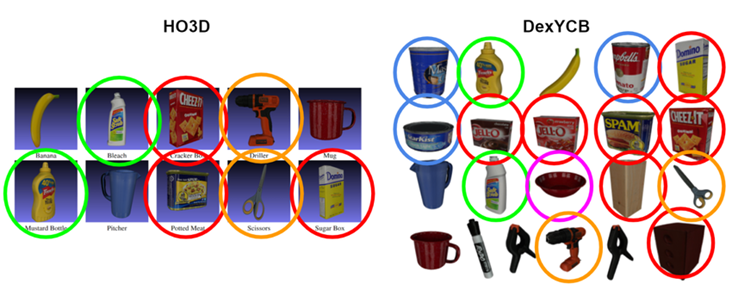
\includegraphics[scale=1]{hoisdf-5.png}
\end{center}

\section*{Future Work}

\subsubsection*{Temporal Consistency for Videos}

While the model is designed for single images, the accuracy can be increased for videos by leveraging temporal constraints. One possible solution is to just pass the final keypoint from the previous frame along with the query point and features to the SDF decoder. This restricts the model from predicting the keypoints in parallel as each frame is dependent on the previous one.

Another solution is to train a separate temporal transformer encoder module, such as TCPFormer~\cite{liu2025tcpformer}, that will receive the keypoint predictions for the video once all the frames have been calculated, and then shifts the keypoints to ensure smooth and consistent transitions. TCPFormer uses an implicit pose proxy to represent pose information, and utilizes self-attention to capture relationships between keypoints across frames.

By incorporating temporal context, keypoints are smoother and more consistent across consecutive frames. Temporal context can also enhance the model's ability to handle occlusions, as information from when a keypoint was visible can help infer the location of the occluded keypoint.

\subsubsection*{Occupancy Fields}

Occupancy fields~\cite{li2024diffusionfof} model 3D shapes by representing the probability that a given a 3D point is inside or outside an object. Unlike signed distance fields, which encode the distance to the surface, occupancy fields classify points based on their occupancy probability, which could handle occlusions better. This approach could replace the SDF decoder in the HOISDF architecture, as it still represents the shape geometry but avoids relying on the exact surface distance. The surface of the hand or object can still be inferred with query points from the occupancy field by determining the decision boundary, where the occupancy probability is at a specific threshold.

\printbibliography[]

\end{document}